\documentclass[letterpaper,10pt]{article}

%\setlength{\parindent}{0in}
%\usepackage{fullpage} 
\usepackage{amsmath}
\usepackage{amssymb}
\usepackage{enumerate}
\usepackage{graphicx}
\usepackage[table]{xcolor}
\usepackage{dcolumn}
\oddsidemargin 0.0in
\textwidth 6.5in
\newcolumntype{.}{D{.}{.}{-1}}
\newcommand*{\myalign}[2]{\multicolumn{1}{#1}{#2}}

%opening
\title{Homework 1}
\author{Steve Mazza}
%\date{January 20, 2012}

\begin{document}
\maketitle

Because I feel like I have a lot of ground to make up, I have attempted all of the problems.  I would very much appreciate any feedback you can provide in the interest of aiding my understanding.

\section*{Problem 1}
There may be a more clever way to do this, but my approach is to find all values for $s$ such that $e^{-as}=1$.  Solving for $s$ we get $s=\dfrac{2i\pi n}{a}$.  There are an infinite number of solutions to this periodic function.
\begin{center}
	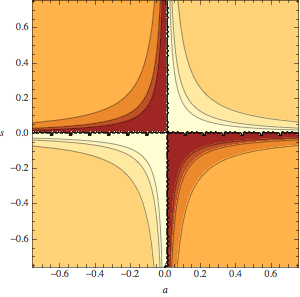
\includegraphics[scale=0.75]{plot.png}
\end{center}

\section*{Problem 2}
The problem describes a step-wise function as follows:
\begin{align}
	f(t) &= T, t\geq T \\
	f(t) &= t, 0 > t > T \\
	f(t) &= 0, t\leq 0
\end{align}
In order to obtain the Laplace transform, the functions must be made continuous.  There are at least two ways to achieve this.  The first is to integrate.
\begin{equation}
	\int_0^T te^{-st} \, \mathrm{d} t + \int_{T}^{\infty} Te^{-st}\, \mathrm{d}t
\end{equation}
The other is to apply the unit step function (let's use this method).
\begin{align}
	f(t) &= t(u(t)-u(t-T))+Tu(t-T) \\
	f(t) &= tu(t)-tu(t-T)+Tu(t-T) \\
	F(s) &= \frac{1}{s^{2}} + \frac{\mathrm{d}}{\mathrm{d}s}\left[e^{-Ts}\frac{1}{s}\right] + T\left(e^{-Ts}\frac{1}{s}\right) \\
	F(s) &= \frac{1}{s^{2}} - \frac{1 - e^{-Ts}\left(Ts+1\right)}{s^{2}} + \frac{T\left(e^{-Ts}\right)}{s} \\
	F(s) &= \frac{1-e^{-Ts}\left(Ts+1\right)}{s^{2}} + \frac{T\left(e^{-Ts}\right)}{s}
\end{align}

\section*{Problem 3}
The partial-fraction expansion is obtained in MATLAB as follows:
\begin{verbatim}
>> num = [1 5 6 9 30];
>> den = [1 6 21 46 30];
>> [r,p,k] = residue(num,den)
\end{verbatim}
\color{lightgray} \begin{verbatim}
r =

  -1.0812 + 1.7051i
  -1.0812 - 1.7051i
  -0.1154 + 0.0000i
   1.2778 + 0.0000i


p =

  -1.0000 + 3.0000i
  -1.0000 - 3.0000i
  -3.0000 + 0.0000i
  -1.0000 + 0.0000i


k =

     1
\end{verbatim} \color{black}
The corresponding formatted equation for the solution is
\begin{equation}
	F(s) = 1 + \frac{-1.0812+1.7051i}{s+1-3i} + \frac{-1.0812-1.7051i}{s+1+3i} + \frac{-0.1154}{s+3} + \frac{1.2778}{s+1}
\end{equation}

The inverse Laplace transform is obtained in MATLAB as follows:
\begin{verbatim}
>> syms s
>> F = (s^4+5*s^3+6*s^2+9*s+30)/(s^4+6*s^3+21*s^2+46*s+30);
>> ilaplace(F)
\end{verbatim}
\color{lightgray} \begin{verbatim}
ans =
 
(23*exp(-t))/18 - (3*exp(-3*t))/26 + dirac(t) - (253*exp(-t)*(cos(3*t) 
	+ (399*sin(3*t))/253))/117
\end{verbatim} \color{black}
The corresponding formatted equation for the solution is
\begin{equation}
	f(t) = \frac{23e^{-t}}{18} 
	- \frac{3e^{-3t}}{26} 
	+ \delta(t) 
	- \dfrac{253e^{-t}\left(\cos(3t) + \dfrac{399\sin(3t)}{253}\right)}{117}
\end{equation}
\emph{Please also see the corresponding MATLAB file for additional work.}

\section*{Problem 4}
\begin{verbatim}
>> z = [-1; -2];
>> p = [0; -4; -6; 2+3i; 2-3i];
>> k = 5;
>> [num,den] = zp2tf(z,p,k);
>> printsys(num,den,'s')
\end{verbatim}
\color{lightgray} \begin{verbatim} 
num/den = 
 
             5 s^2 + 15 s + 10
   ------------------------------------
   s^5 + 6 s^4 - 3 s^3 + 34 s^2 + 312 s
\end{verbatim} \color{black}
The corresponding formatted equation for the solution is
\begin{equation}
	F(s)=\dfrac{5 s^2 + 15 s + 10}{ s^5 + 6 s^4 - 3 s^3 + 34 s^2 + 312 s}
\end{equation}
\emph{Please also see the corresponding MATLAB file for additional work.}

\section*{Problem 5}
We are asked to first derive the inverse Laplace transform of the function $F(s) = \dfrac{5}{s^2\left(s^2+\omega^2\right)}$ by hand.
\begin{align}
	F(s) &= \dfrac{5}{s^2\left(s^2+\omega^2\right)} \\
	F(s) &= \dfrac{5}{\omega^3}\left(\dfrac{\omega^3}{s^2\left(s^2+\omega^2\right)}\right) \\
	f(t) &= \left(\dfrac{5}{\omega^3}\right)\omega t-\sin(\omega t) \\
	f(t) &= \dfrac{5\omega t-5\sin(\omega t)}{\omega^3}
\end{align}
Next we find the solution using MATLAB.
\begin{verbatim}
>> syms w
>> F = 5/(s^2*(s^2+w^2));
>> ilaplace(F)
\end{verbatim}
\color{lightgray} \begin{verbatim} 
ans =
 
(5*t)/w^2 - (5*sin(t*w))/w^3
\end{verbatim} \color{black}
The corresponding formatted equation for the solution is
\begin{equation}
	f(t) = \dfrac{5t}{\omega^2} - \dfrac{5\sin(t\omega)}{\omega^3}
\end{equation}
\emph{Please also see the corresponding MATLAB file for additional work.}

\section*{Problem 6}
We apply the technique described in the introduction handout.
\begin{center}
	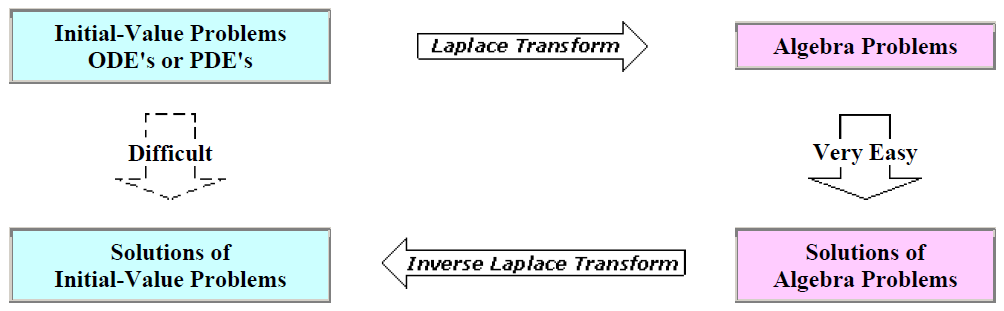
\includegraphics[scale=0.5]{process.png}
\end{center}
\begin{align}
	s^2F(s) - s(-1)-2+3(sF(s)-(-1))+2F(s) &= 0 \\
	F(s)(s^2+3s+s) &= -(s+1) \\
	F(s) &= \dfrac{-(s+1)}{s^2+3s+2} \\
	F(s) &= -\dfrac{1}{s+2} \\
	f(t) &= -e^{-2t}
\end{align}
I also provide a solution computed directly through MATLAB:
\begin{verbatim}
>> dsolve('D2x+3*Dx+2*x=0','x(0)=-1, Dx(0)=2')
\end{verbatim}
\color{lightgray} \begin{verbatim} 
ans =
 
-exp(-2*t) 
\end{verbatim} \color{black}
\emph{Please also see the corresponding MATLAB file for additional work.}

\end{document}